\chapter{Visualization of seasonal influenza A/H3N2 experimental phenotypes}

\section{dms-view: Interactive visualization tool for deep mutational scanning data}

With the exception of subsection~\ref{subsec:visual-design-decisions}, this work was originally published in \emph{The Journal of Open Source Software} at \url{https://doi.org/10.21105/joss.02353}.

\subsection{Summary and Purpose}

The high-throughput technique of deep mutational scanning (DMS) \citep{fowler2014deep} has recently made it possible to experimentally measure the effects of all amino-acid mutations to a protein (Figure~\ref{fig:dms}).
Over the past five years, this technique has been used to study dozens of different proteins \citep{esposito2019mavedb} and answer a variety of research questions.
For example, DMS has been used for protein engineering \citep{wrenbeck2017deep}, understanding the human immune response to viruses \citep{Lee2019}, and interpreting human variation in a clinical setting \citep{starita2017variant,gelman2019recommendations}.
Accompanying this proliferation of DMS studies has been the development of software tools \citep{bloom2015software,rubin2017statistical} and databases \citep{esposito2019mavedb} for data analysis and sharing.
However, for many purposes it is important to integrate and visualize the DMS data in the context of other information, such as the 3-D protein structure or natural sequence-variation data.
Currently, this visualization requires the use of multiple different tools including custom scripts, static visualization tools like MaveVis \citep{esposito2019mavedb}, or protein structure software such as PyMol \citep{PyMOL}.
No existing tools provide linked views of the protein structure and DMS data in a single interface to facilitate dynamic data exploration and sharing.

\begin{figure}
  \centering
  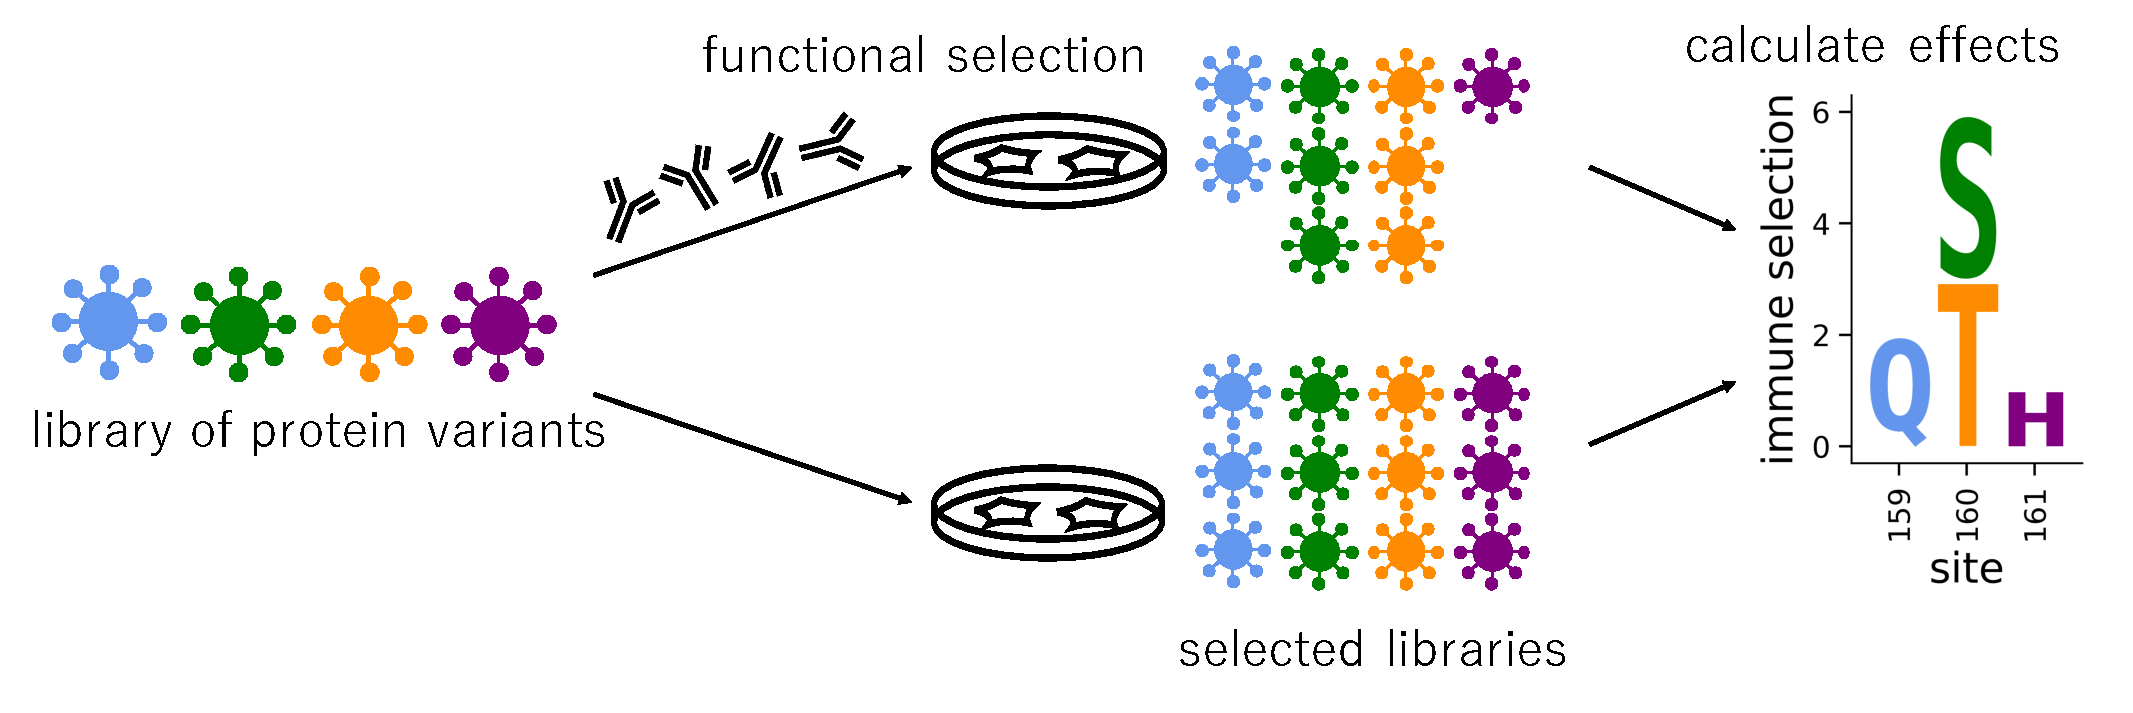
\includegraphics[width=\textwidth]{chapter_03/dms.pdf}
  \caption{Example deep mutational scanning workflow, modified from \citet{Lee2019}. The goal of this experiment is to quantify the how mutations affect a virus's ability to escape an antibody. The viral variant library contains all single amino-acid changes away from wildtype. The viral library is passaged in cell culture, with and without antibodies, to select for functional variants. Mutational effects are calculated based on deep sequencing of the pre-selected and post-selected libraries.\label{fig:dms}}
\end{figure}

Here we describe \emph{dms-view} (https://dms-view.github.io/), a flexible, web-based, interactive visualization tool for DMS data.
\emph{dms-view} is written in JavaScript and \href{https://d3js.org}{D3}, and links site-level and mutation-level DMS data to a 3-D protein structure.
The user can interactively select sites of interest to examine the DMS measurements in the context of the protein structure.
\emph{dms-view} tracks the input data and user selections in the URL, making it possible to save specific views of interactively generated visualizations to share with collaborators or to support a published study.
Importantly, \emph{dms-view} takes a flexible input data file so users can easily visualize their own DMS data in the context of protein structures of their choosing, and also incorporate additional information such amino-acid frequencies in natural alignments.

\begin{figure}
  \centering
  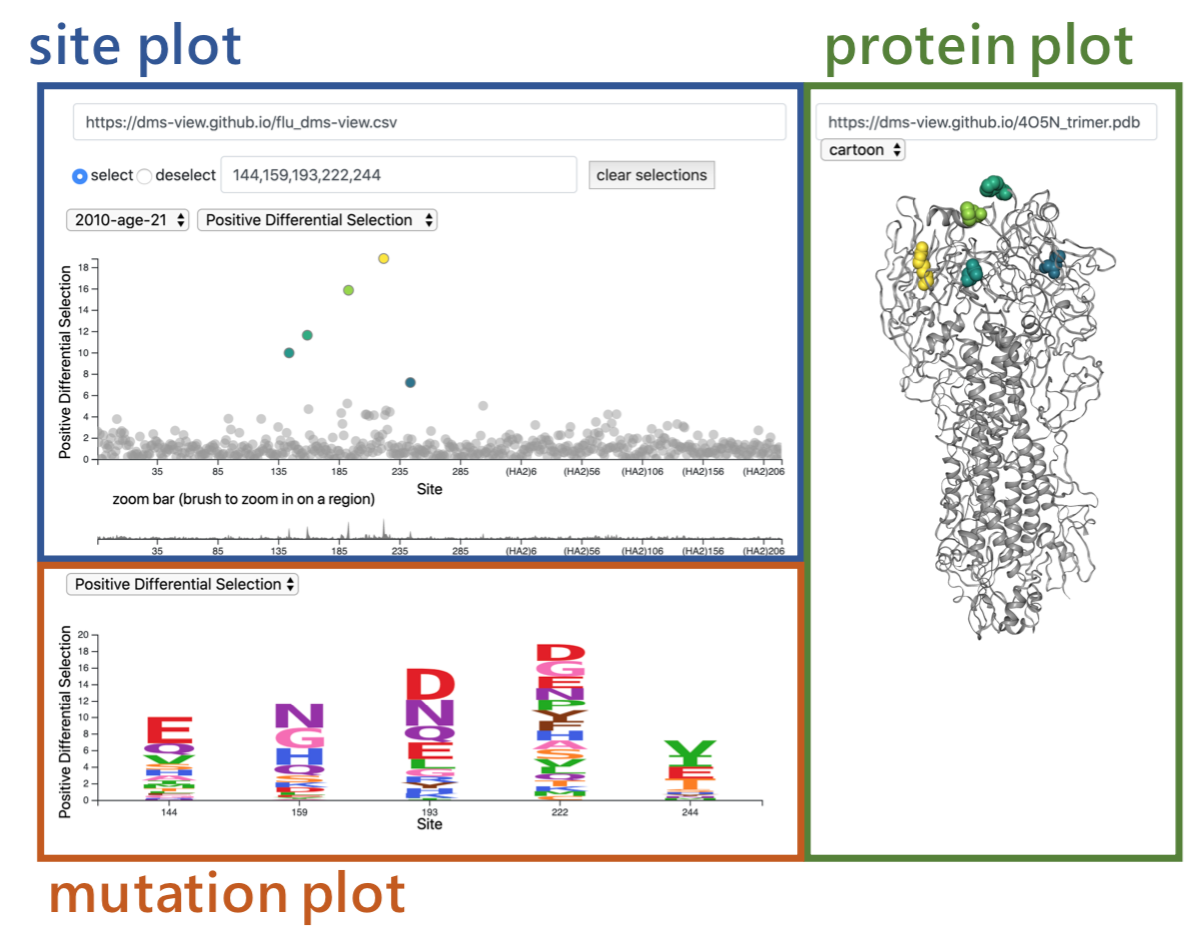
\includegraphics[width=\textwidth]{chapter_03/dms-view-layout.png}
  \caption{\label{fig:dms-view-layout}Using \emph{dms-view} to analyze DMS data.
    For further exploration, please visit https://dms-view.github.io.
    The \emph{dms-view} data section has three panels: the site plot, the mutation plot, and the protein structure plot.
    The interactive features for selecting sites and navigating are in the site plot panel.
    Here we show the five sites most highly targeted by human serum ``2010-Age-21'' from the study by \citet{Lee2019}.
    All five sites fall in the ``globular head'' of influenza virus HA.}
\end{figure}

\begin{figure}
  \centering
  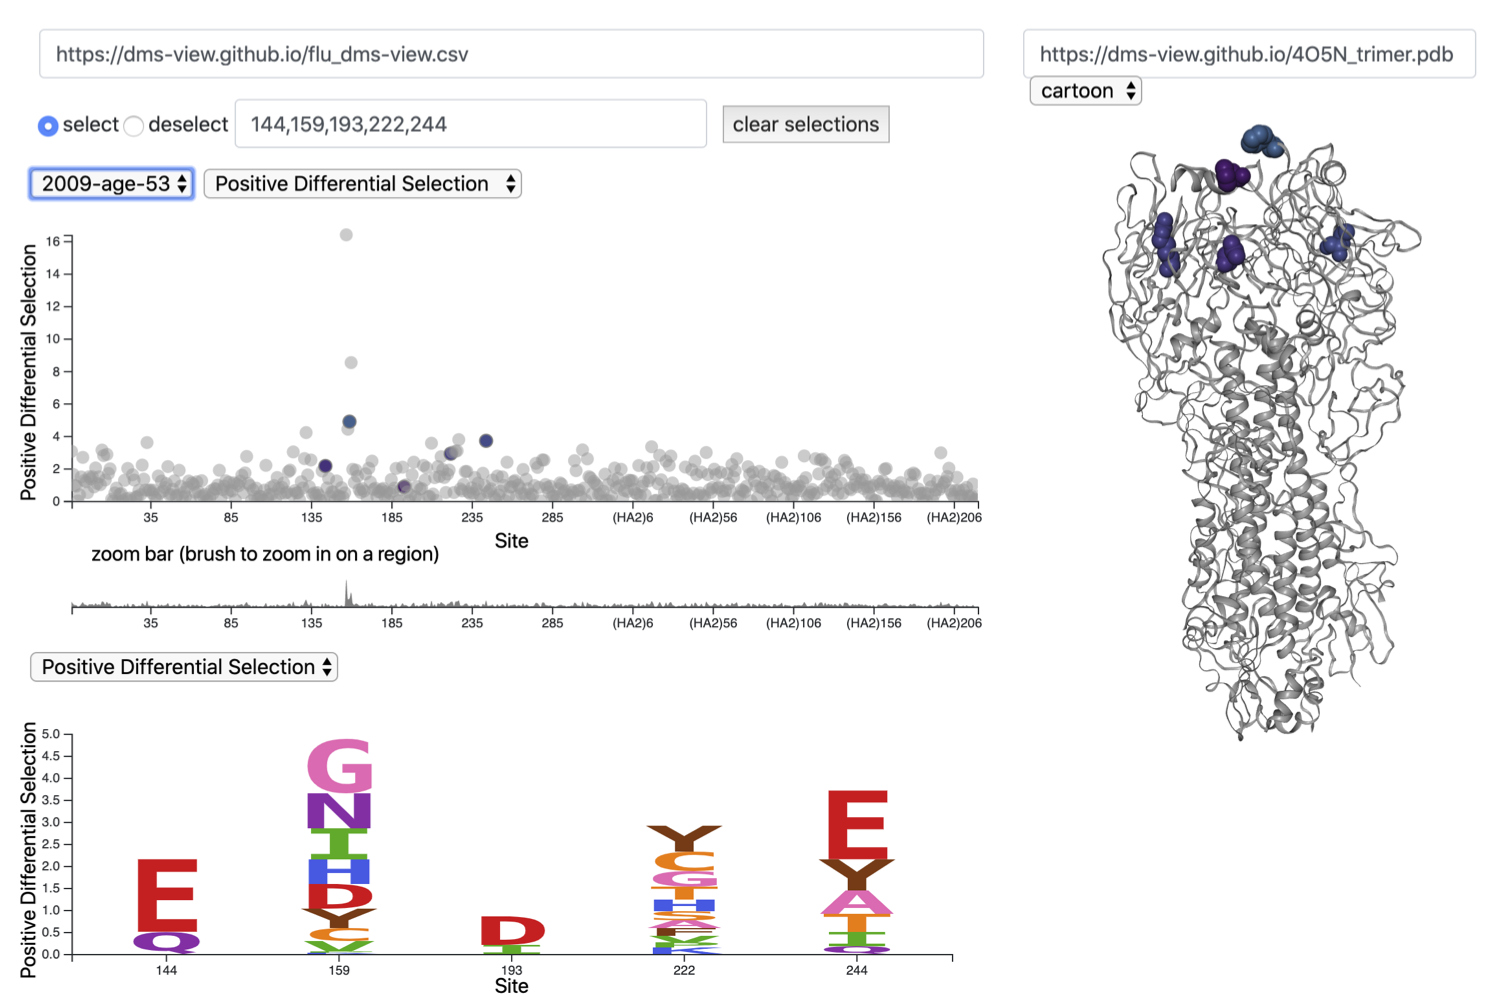
\includegraphics[width=\textwidth]{chapter_03/dms-view-variation-by-serum.png}
  \caption{\label{fig:dms-view-variation-by-serum} The same five sites as in Figure~\ref{fig:dms-view-layout} but now plotted with the data from a different human serum, ``2009-age-53''.
    Using \emph{dms-view} to compare, we see that different sites on HA are targeted by different sera.}
\end{figure}

Users can access \emph{dms-view} at https://dms-view.github.io.
The tool consists of a data section at the top and a description section at the bottom.
The data section displays the user-specified data in three panels: the site-plot panel, the mutation-plot panel, and the protein-structure panel (Figure~\ref{fig:dms-view-layout}).
When sites are selected in the site-plot panel, the individual mutation values are shown in the mutation-plot panel and highlighted on the protein structure.
The user can toggle between different conditions, site- and mutation-level metrics, all of which are defined in the user-generated input file.
The description section is at the bottom of the page, and allows the user to add arbitrary notes that explain the experimental setup, acknowledge data sources, or provide other relevant information.
Note that dms-view is designed to visualize the effects of single mutations, not combinations of mutations.

Please visit the documentation at https://dms-view.github.io/docs to learn more about how to use the tool, how to upload a new dataset, or view case studies.

\subsection{Case study: mapping influenza A virus escape from human sera}

Using a DMS approach, \citet{Lee2019} measured how all amino-acid mutations to the influenza virus surface-protein hemagglutinin (HA) affected viral neutralization by human sera.
For more information on the experimental setup, see the paper \citep{Lee2019} or the GitHub repository (\url{https://github.com/jbloomlab/map_flu_serum_Perth2009_H3_HA}).

We visualized the \citet{Lee2019} serum mapping data using \emph{dms-view}.
To explore this dataset, please visit https://dms-view.github.io.
In the \emph{dms-view} visualization of these data, the conditions are the different human sera used for the selections.
The site- and mutation-level metrics are different \href{https://jbloomlab.github.io/dms_tools2/diffsel.html}{summary statistics} measuring the extent that mutations escape from immune pressure.

Lee and colleagues asked two questions in their paper which can be easily explored using \emph{dms-view}.
First, are the same sites selected by sera from different people?
To explore this question, we compared the site-level and mutation-level metric values for a specific set of sites between different conditions.
Second, where on the protein structure are the highly selected sites located?
To explore this question, we selected specific sites of interest to be visualized on the 3-D protein structure.

\subsubsection{Comparing site-level and mutation-level metric values for specific sites between conditions}

To address whether or not the same sites are selected by different human sera using \emph{dms-view}, we highlighted the most highly targeted sites for the human sera condition ``Age 21 2010'' in Figure~\ref{fig:dms-view-layout} (144, 159, 193, 222, and 244).
We then used the condition dropdown menu to toggle to the other sera.
The highlighted sites remain highlighted after the condition is changed so we can easily see if the same sites are targeted in other conditions.

In Figure~\ref{fig:dms-view-variation-by-serum}, we can see that there is no overlap of the sites selected by the human sera ``2010-age-21'' and the human sera ``2009-age-53''.
These data are the default data for \emph{dms-view}, so to explore this question in more detail please see https://dms-view.github.io.

\subsubsection{View sites on the protein structure}

To address where on the protein structure the targeted sites are located, we selected the most highly targeted sites (144, 159, 193, and 222) for the human sera condition ``Age 21 2010'' to highlight them on the protein structure.

In Figure~\ref{fig:dms-view-layout}, we can see that these sites cluster on the ``head'' of HA, which is known to be a common target of the human immune system \citep{Chambers:2015jt}.

\subsection{Code availability}

\emph{dms-view} is available at \url{https://dms-view.github.io}.
Source code is available at \url{https://github.com/dms-view/dms-view.github.io}.
Documentation is available at \url{https://dms-view.github.io/docs} and case studies are available at \url{https://dms-view.github.io/docs/casestudies/}.

\subsection{Visual design decisions behind dms-view}
\label{subsec:visual-design-decisions}

With one notable exception, we designed \emph{dms-view} to use the most expressive and effective representations of the underlying data.
Expressiveness describes the ability of a visualization to communicate the most relevant information in a dataset, while effectiveness describes how rapidly a viewer can perceive the relevant information \citep{Mackinlay1986}.
Expressive and effective visualizations require the designer to select appropriate representations of the data based on the designer's understanding of human perception, available modes of representation, and the data being visualized.

To these ends, we selected encodings of DMS data that were most appropriate for these data.
In the ``site plot'', we represented quantitative values as circles on a discrete genomic coordinate scale of the x-axis and a continuous scale on the y-axis.
We chose a redundant color encoding of the site metric values to both emphasize the differences between multiple selected values and to link selected sites in the ``site plot'' with their placement on the protein structure.
We colored unselected points gray to communicate their position in the site plot and distinguish them from selected points with color.
We used reduced opacity for unselected points, to reduce occlusion caused by overlapping circles and maintain a reasonable circle size for user interactions.
We increased the expressiveness of site plot data by providing details on demand that users can access by hovering over specific points.
We increased the effectiveness of site plot data by adding filter, zoom, and select interactions that allow the user to reduce the number of data points to inspect at any given time.

In the ``mutation plot'', we used the same approach of representing quantitative data on a discrete genomic coordinate scale and a continuous ``mutation metric'' scale.
In contrast to the site plot, we chose to only show mutation-level data for sites that users selected in the site plot.
We also chose to represent these quantitative data by the height of the alphabetical letter associated with the amino acid of the mutation at each position.
This encoding, also known as a ``logo plot'', allowed us to communicate additional information about the relative contribution of each amino acid to an overall site metric.
Although logo plots are technically a less effective representation of these quantitative data, due to their use of arbitrary differences in area associated with each letter, they are a standard representation of these data in the field of DMS research.
We applied a color encoding to each mutation metric value such that amino acids were colored according to their biophysical group (hydrophobic, positively charged, negatively charged, etc.).
As with the site plot, we provided details on demand when the user hovers over specific mutations at each genomic position.
A major limitation of our logo plot implementation is its fixed width.
As the user selects more sites in the site plot, we scale down the width of each logo plot column.
When more than a couple dozen sites have been selected, the amino acid letters in the logo plot become illegible for all except the higher values.

Finally, we encoded the 3D structure of a given protein using a reduced space representation known as the ``cartoon'' view.
In this view, selected sites appear more clearly as large bubbles against a ribbon of the unselected sites.
We enabled the protein viewer's rotation functionality that allows users to spin the protein around in three dimensions.
As with the site plot, we encoded the site metric of each position by color on a viridis scale.
We made this choice primarily because the most effective representations of these quantitative data (the spatial x, y, and z axes) were already in use by the protein structure itself.
We also provided details on demand for each protein site.

\section{Visualization of antigenic phenotypes}

\subsection{Introduction}

A primary component of seasonal influenza A/H3N2 evolution is the ability of viruses to acquire mutations that allow them to escape antibodies from previous infections.
This process, known as antigenic drift, changes the appearance of viral surface proteins hemagglutinin (HA) and neuraminidase (NA).
Viruses balance escape from antibodies with the maintenance of their protein functions.
The HA surface protein allows viruses to bind to the surface of new host cells and initiate infection.
When antibodies bind to HA, they can prevent viruses from binding and infecting cells.
Viruses that acquire mutations to HA that prevent antibodies from binding but do not disrupt the ability of HA to bind to host cells should be able to infect hosts.

Experimental measurements of antigenic drift allow researchers to quantify how well viruses with different HA mutations can escape detection by antibodies.
Until recently, the most reliable of these experimental measurements were hemagglutination inhibition (HI) assays \citep{hirst1943studies}.
In these assays, researchers place red blood cells into a multi-well plate and add one test virus per well.
When a well contains only blood cells and virus, the virus binds to the blood cells causing them to agglutinate into a wide, red dot that fills the well.
Next, researchers add two-fold dilutions of antisera from naive ferrets that were infected by a single reference virus.
When the antisera contains enough antibodies to effectively bind the virus, the blood cells do not agglutinate and instead sink to the bottom of the well in a small red dot.
The highest dilution of antisera required to inhibit agglutination provides the ``titer'' measurement between the reference and test viruses.
When the test virus is the same as the reference virus, the assay provides an autologous titer measurement.
When the test and reference viruses differ, the assay provides a heterologous titer measurement.

Researchers report titer measurements as both raw and normalized values.
Raw titer measurements represent the denominator associated with the minimum dilution required to inhibit agglutination.
These two-fold dilution series have raw measurements like 80, 160, 320, etc. such that lower numbers represent the presence of more antisera in the dilution.
These raw measurements can also be represented more conveniently on a $\log_{2}$ scale \citep{Smith:2004jc,Bedford:2014bf}.
Antisera vary in their potency such that some sera always require higher or lower dilutions to inhibit agglutination regardless of the test virus.
For example, a low potency antiserum requires a lower dilution to inhibit agglutination by the same reference virus resulting in a low autologous titer.
To account for this variable potency, we normalize titer measurements by subtracting the $\log_{2}$ titer between a test and reference virus (the heterologous titer) from the $\log_{2}$ titer between the reference virus and its own antisera (the autologous titer).
The resulting normalized titers enable comparisons of antigenic distances across reference viruses.
Importantly, viruses with a $\log_{2}$ distance greater than 2 are considered antigenically distinct for the purposes of deciding updates to vaccine composition \citep{}.

\subsection{Previous visual representations of antigenic distances}

To understand broad patterns of antigenic drift beyond simple pairwise relationships, antigenic distance must be summarized by statistical or visual representations.
For example, the method of antigenic cartography maps multidimensional antigenic distances to a two-dimensional space using dimensionality reduction methods \citep{Smith:2004jc,Bedford:2014bf}.
These map-like visualizations reveal long-term patterns and trends in antigenic drift within seasonal influenza lineages like the punctuated emergence of new antigenic clusters every few years (Figure~\ref{fig:antigenic-cartography-bedford-2014}).
However, antigenic cartography is less suited to representations of short-term antigenic drift on the same time scale as annual vaccine updates in each hemisphere.

\begin{figure}
  \centering
  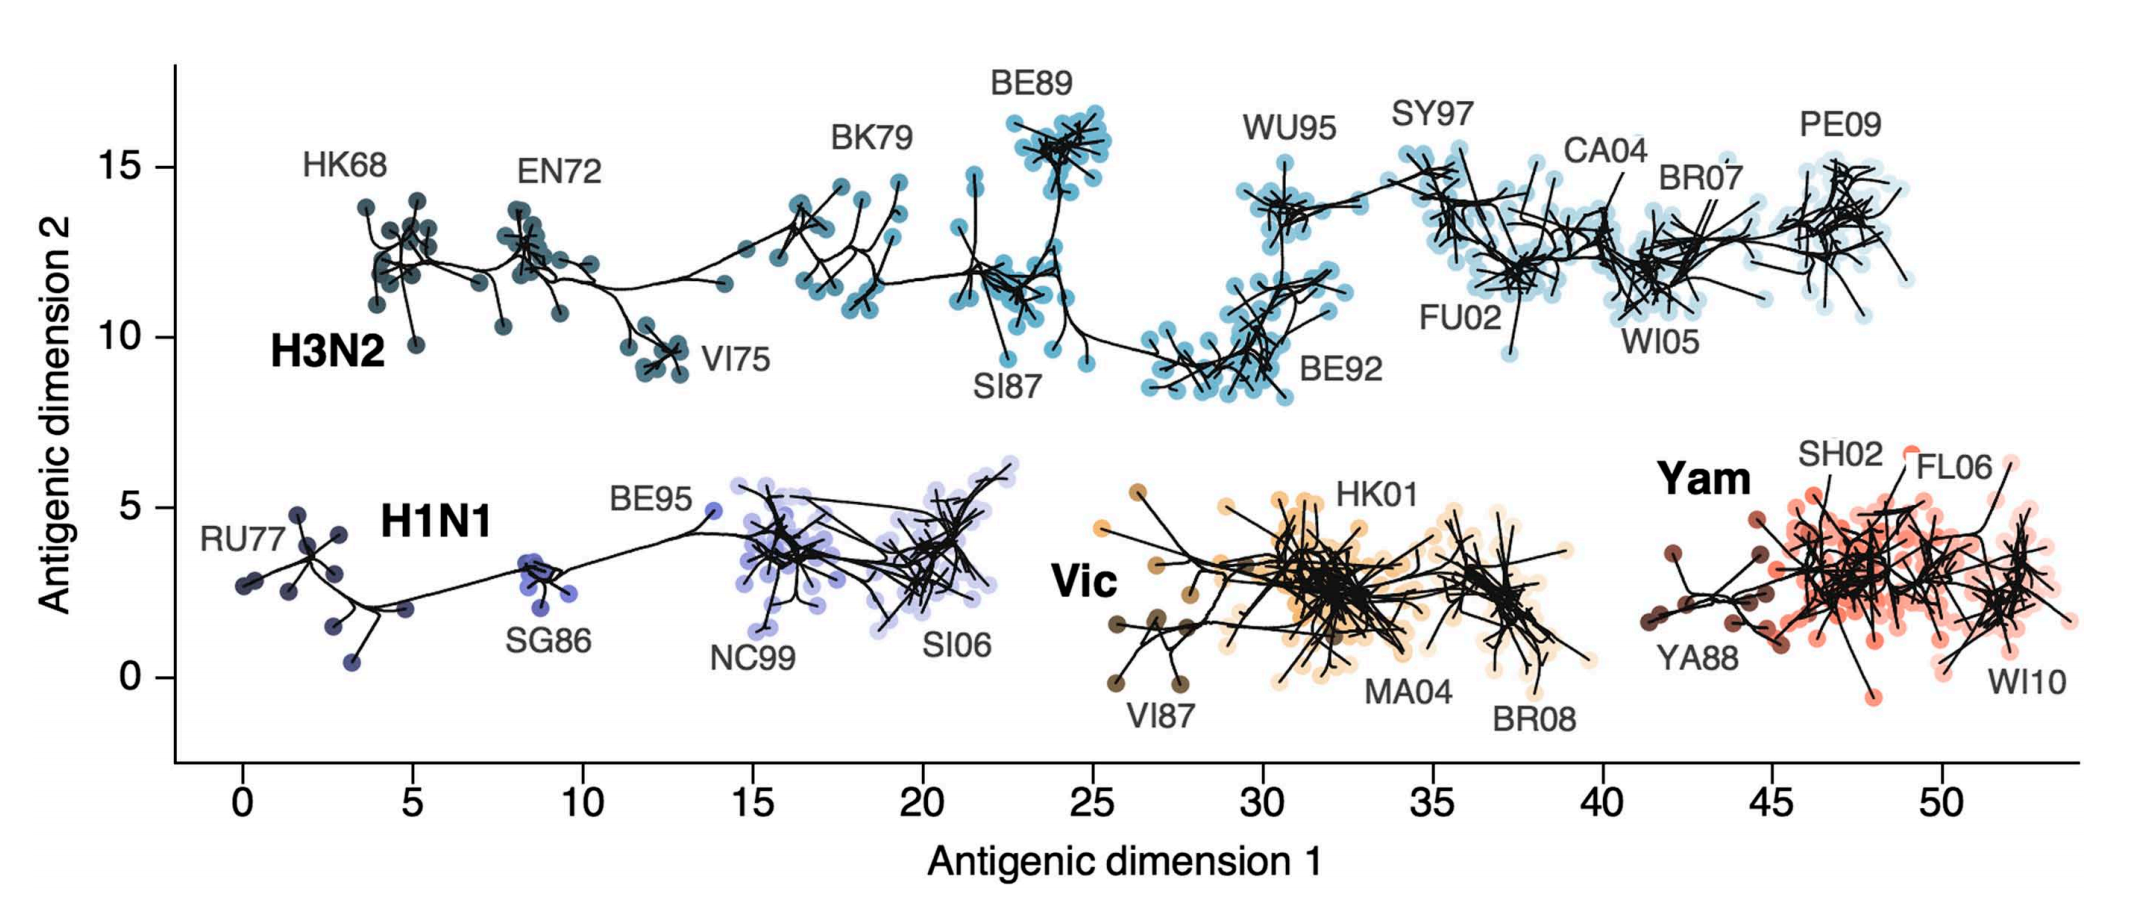
\includegraphics[width=\textwidth]{chapter_03/antigenic-cartography-bedford-2014.png}
  \caption{\label{fig:antigenic-cartography-bedford-2014} Antigenic cartography of titer measurements from seasonal influenza lineages from Figure 1 of \citet{Bedford:2014bf}.
    Raw titer measurements in a multidimensional matrix are transformed through Bayesian multidimensional scaling (BMDS) to a two-dimensional representation.
    These antigenic maps reveal long-term patterns of antigenic drift.}
\end{figure}

Alternate visualizations created in the nextflu \citep{Neher:2015jr} and Nextstrain \citep{Hadfield2018} frameworks address the needs of influenza researchers who make decisions about vaccine composition.
Within nextflu, all available pairwise antigenic distances between a selected reference virus's antisera and test viruses are represented by colored tips on a phylogenetic tree constructed from HA sequences (Figure~\ref{fig:titer-phylogeny}).
This interactive visualization allows users to select a specific reference virus by clicking a ``gear'' icon drawn on the phylogeny where the reference virus occurs.
All tips in the tree that have titer measurements to the selected reference appear as circles colored by the quantitative value of their antigenic distance (e.g., smaller distances are blue, larger distances are red).
This representation of the pairwise data allows users to identify phylogenetic clades that are antigenically distance from a given antiserum or that are missing measurements from that antiserum.
Influenza virologists use this information to select potential vaccine candidates that ``cover'' the most extant clades and prioritize which HI assays to perform next.
The benefits of visualizing the phylogenetic context of antigenic distances for a single antiserum are balanced by visual design costs of not showing antigenic distances for all antisera in a single view.

\begin{figure}
  \centering
  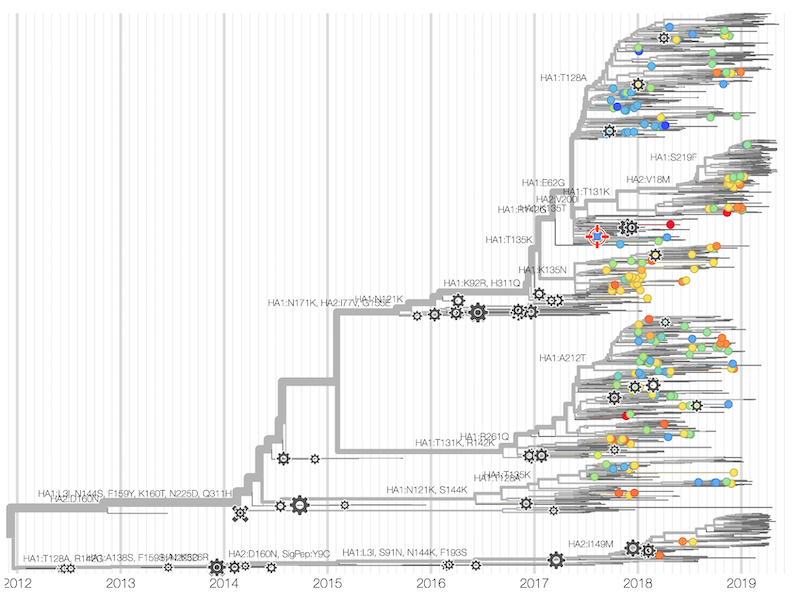
\includegraphics[width=\textwidth]{chapter_03/nextflu-titer-phylogeny.png}
  \caption{\label{fig:titer-phylogeny} Antigenic distance (mean $\log_{2}$ titer drop) between test strains (colored tips) and a selected reference virus's antiserum (red crossmark) in the context of a H3 phylogeny of recently circulating strains from nextflu \citep{Neher:2015jr}.}
\end{figure}

Another recent representation of pairwise antigenic distances attempts to address the limitations of the phylogenetic visualization.
This representation summarizes the mean antigenic distances between a subset of relevant reference viruses (i.e., likely vaccine candidates) and all tests viruses within each extant clade.
The resulting heatmaps use the x-axis to encode phylogenetic clades, the y-axis to encode reference viruses, and color to encode the mean $\log_{2}$ distance between a given reference virus and corresponding test viruses (Figure~\ref{fig:titer-matrix}).
These static heatmaps express more data than the phylogenetic representation, allowing decision-makers to identify qualitative trends across antisera and clades in biannual reports to the World Health Organization \citep{Bedford271114,Bedford780627}.
As with all heatmap, these titer matrices suffer reduced expressiveness by encoding the most valuable quantitative data with color instead of a spatial scale.

\begin{figure}
  \centering
  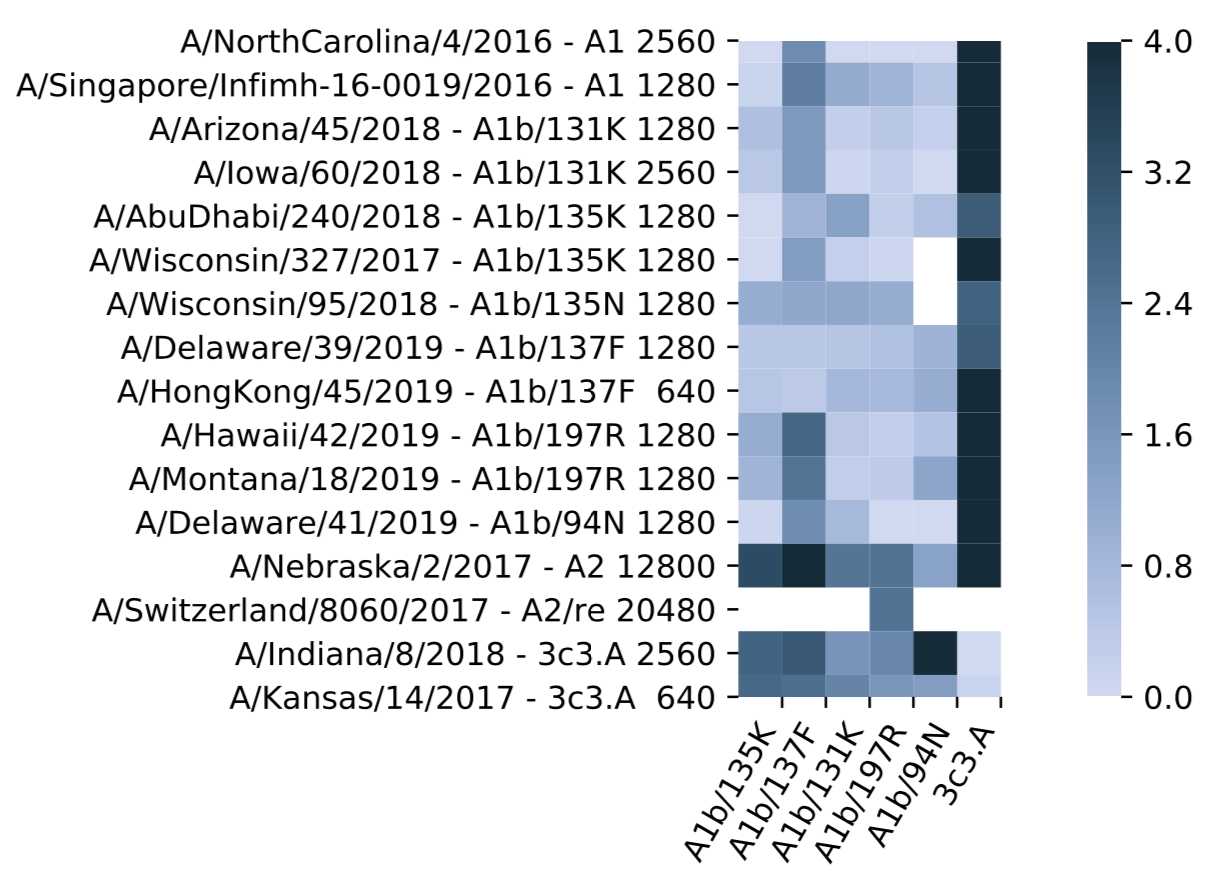
\includegraphics[width=\textwidth]{chapter_03/titer_matrix_who_h3n2_ha_2y_cell_hi.png}
  \caption{\label{fig:titer-matrix} Antigenic distance (mean $\log_{2}$ titer drop) between test strains sampled from recently circulating clades (columns) and antisera for representative viruses from these clades (rows).
    The median autologous raw titer of antisera for representative viruses is shown after the corresponding virus's name and clade membership.
    White squares represent missing data.}
\end{figure}

\subsection{Improved visual representations of antigenic distances}

Given the benefits and costs of existing visualizations of antigenic distances, we wondered whether we could apply user-driven design and established visual design principles to produce a more expressive and effective visualization for influenza virologists.
To this end, we established the goals of users who would interact with our visualizations, identified the most effective encodings for the data users needed to explore, and composed an interactive visualization from these encodings to address the desired goals.

Based on informal user interviews with collaborators at the Influenza Division of the Centers for Disease Control and Prevention, we identified a list of primary goals for the phylogenetic and heatmap visualizations.
Users wanted to know which currently circulating clades of influenza have measurements against a given serum, to prioritize which clades to select test viruses from in future HI experiments.
Additionally, users wanted to know which available antiserum has the lowest antigenic distance across all circulating clades, to identify potential vaccine candidates.
Finally, users wanted to compare the antigenic diversity of extant clades.
From these user goals, we decided that an optimal visualization would summarize the distribution of antigenic distances by antiserum and clade.

We observed that the existing titer matrix heatmaps addressed most of the user goals except for communicating which extant clades were missing measurements.
Both the phylogenetic and heatmap views use color to encode the most relevant quantitative data of antigenic distance.
Previous visualization design research has shown that quantitative data are more effectively represented by positional encodings (e.g., x- or y-axis positions) whereas nominal data (e.g., phylogenetic clades) can be effectively encoded with color \citep{Mackinlay1986}.
In the phylogenetic view, the two available positional axes are used to represent time and the unitless phylogenetic position of nodes.
Neither of these data are relevant to the user goals described above.
In the titer matrix heatmaps, the two positional axes are used to encode two nominal data types (reference virus name and clade name).

We reasoned that we could make a more effective visualization that addressed most user goals by changing the encoding of data in the titer matrix heatmaps.
Specifically, we chose to temporally omit clade names from the visualization and encode the antigenic distances on the positional x-axis.
By encoding antigenic distance on a positional axis, we could annotate relevant thresholds for antigenic distances, show all available measurements for each reference virus at once, and display a summary statistic (mean antigenic distance) for each reference virus.
We chose to maintain the encoding of nominal reference virus names on the y-axis, since most user goals require interrogation of specific antisera.
With color available as an additional channel, we decided to encode the antigenic class of each antigenic distance with color.
We implemented this design as an interactive visualization with the Altair visualization framework \citep{VanderPlas2018} at \url{https://cse512-19s.github.io/A3-Influenza-vaccine/} (Figure~\ref{fig:prototype-antigenic-viz}).

\begin{figure}
  \centering
  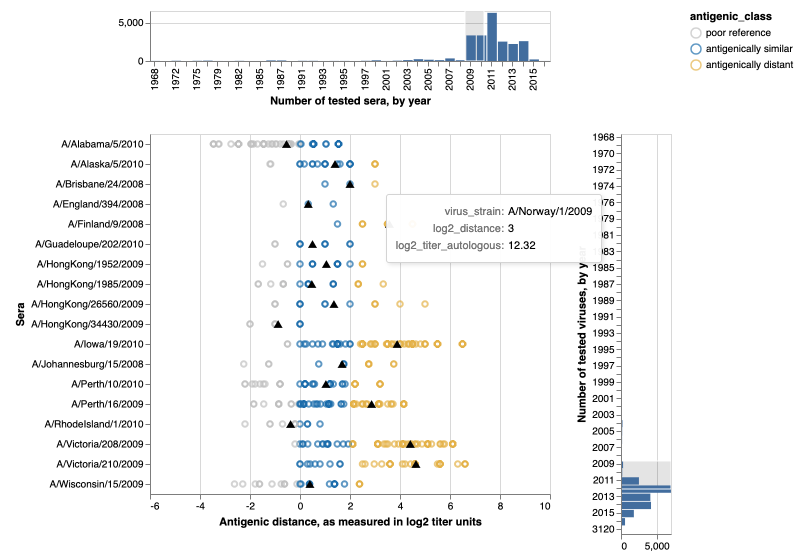
\includegraphics[width=\textwidth]{chapter_03/prototype-antigenic-viz.png}
  \caption{\label{fig:prototype-antigenic-viz} Antigenic distance (mean $\log_{2}$ titer drop) between test viruses (circles) by serum reference virus.
    Colors indicate distances at different actionable thresholds including measurements with a poor reference titer measurement (gray), measurements above two $\log_{2}$ units indicating substantial antigenic drift (yellow), and all other measurements (blue).
    Black triangles show the mean antigenic distance per serum.
    Histograms at the top and right represent the number of sera or test viruses per year, respectively.
    The interactive version of the visualization allows users to filter distances reported to a range of years for sera and test viruses by clicking and dragging across the corresponding histogram.
    The interactive visualization provides details on demand when users hover over specific circles including the name of the test virus, the $\log_{2}$ distance between test and reference viruses, and the $\log_{2}$ autologous distance of the corresponding serum.
  }
\end{figure}

This interactive visualization allows users to quickly compare which antisera have more measurements than others by the presence or absence of circles.
By interactively selected years of test viruses to display, users can filter the display to see the distribution of antigenic distances (and mean distance) to recent viruses from all selected antisera.
The distribution of antigenic distances identifies which antisera have perform poorly in HI assays (those with many negative normalized values, shown in gray) and which are antigenically distinct from most circulating viruses (i.e., poor vaccine candidates).

Despite its strengths, this visualization also has several weaknesses.
Distances are not grouped anywhere by clade, making comparisons between antisera by clade impossible.
This missing information also prevents users from identifying which clades need more titer measurements.
Finally, the alphabetic order of reference viruses on the y-axis wastes an opportunity to communicate more important information to the user.
For example, if users could choose to sort the reference viruses by their mean antigenic distance or by their number of measurements, this single visualization could help users more rapidly identify antisera to consider for vaccine candidates or for additional HI experiments.
We anticipate that the inclusion of clade status in a future implementation (by color or in small multiples) and the default sorting of reference viruses by mean antigenic distance could address these remaining limitations (for example, Figure~\ref{fig:mockup-of-antigenic-distance-by-clade}).
The resulting visualization could provide a more effective real-time view of the same data currently displayed statically in titer matrix heatmaps.

\begin{figure}
  \centering
  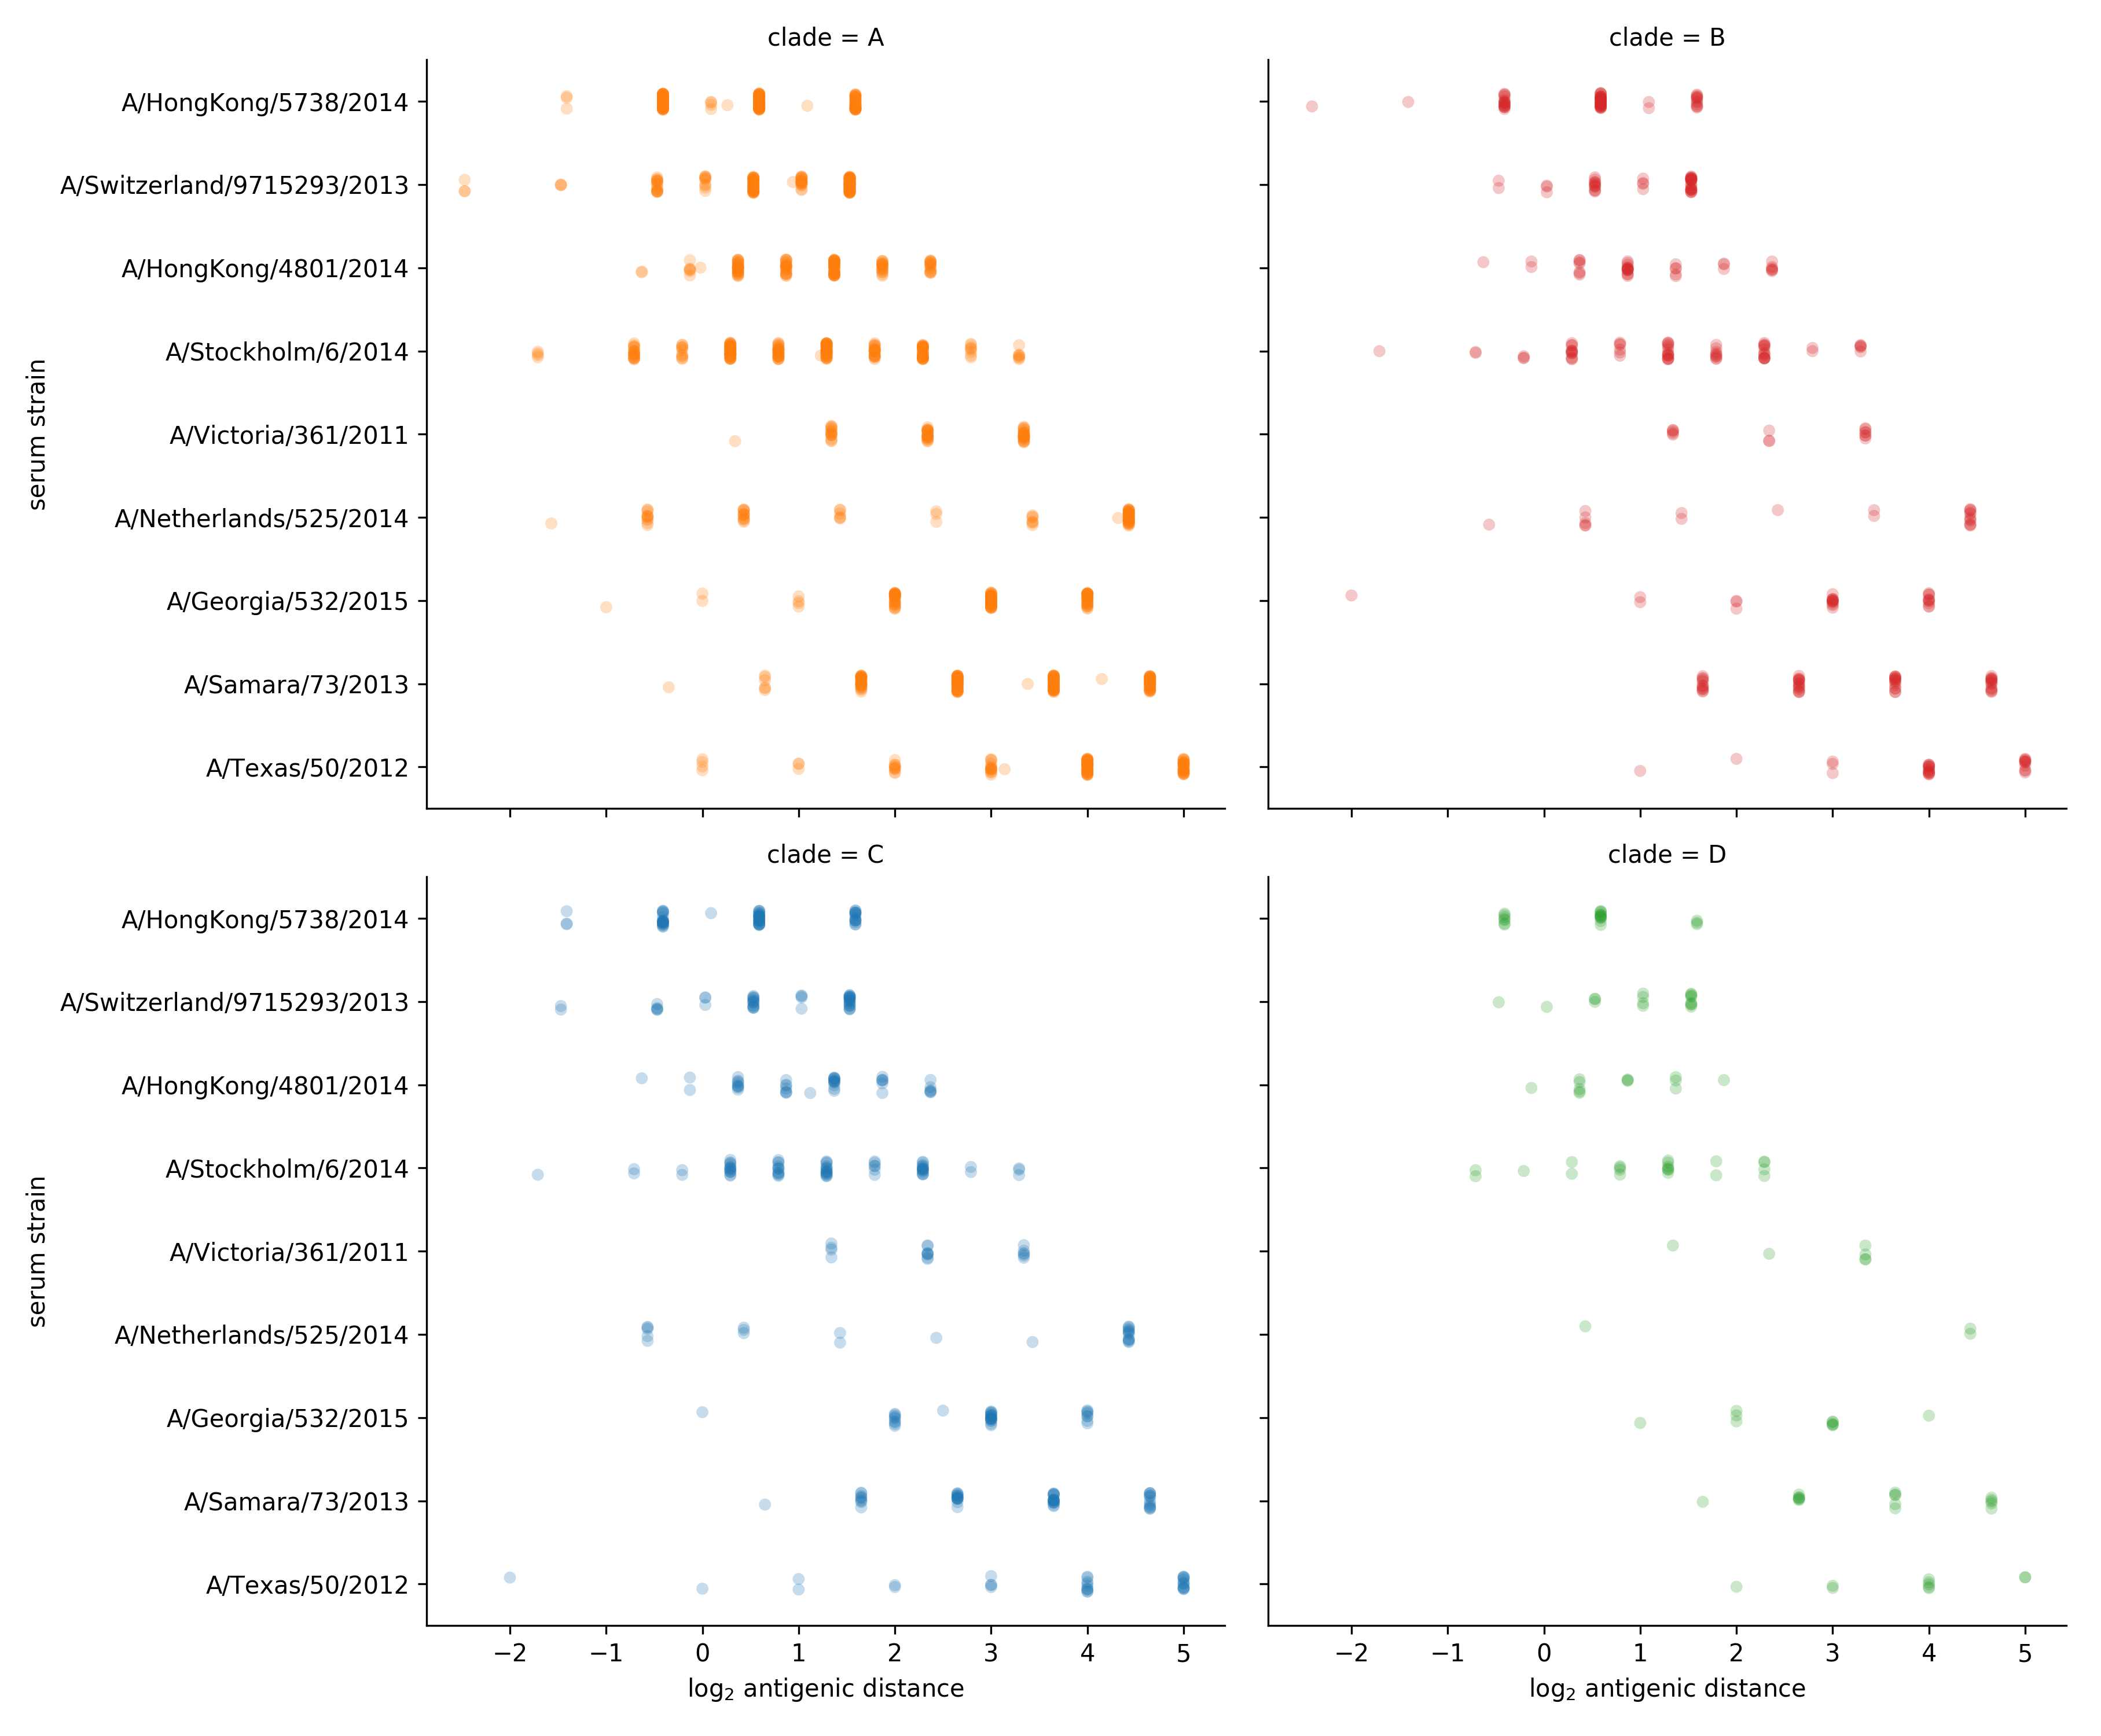
\includegraphics[width=\textwidth]{chapter_03/antigenic-distance-by-clade-and-serum-mockup.png}
  \caption{\label{fig:mockup-of-antigenic-distance-by-clade} Mockup of an alternative representation of antigenic distances by clade and antiserum.
  This encoding of data would allow users to accomplish primary goals including identifying antisera without many measurements, distance of reference viruses across clades, and comparison of antigenic distances between clades.}
\end{figure}
